
Let $(\mathcal{F}, d)$ be a metric space and
$(\mathcal{X}_i, {Y}_i)_{i \le i \le n}$ a training set with their
respective labels or responses.
To estimate a datum $x$, either for classification or prediction of its
response, firstly, it will be necessary to find the elements of the training set
closest to this datum, which will form its neighborhood, denoted as $k(x)$.

There are two variants of these methods. In the first one, consisting of
k-nearest neighbors estimators, it is taken as neighborhood the $k$ closest
elements to $x$, i. e., if the training pairs are re-indexed as
$(\mathcal{X}_{(i)}, Y_{(i)}) \, 1\le i\le n$ so that the
$\mathcal{X}_{(i)}$'s are re-arranged in increasing distance from $x$,
$d(x, \mathcal{X}_{(1)}) \le d(x, \mathcal{X}_{(2)}) \le \dots \le d(x, \mathcal{X}_{(n)})$,
 then $k(x) = \{\mathcal{X}_{(i)} \, : \, 1 \le i \le i\le k\}$.

\begin{figure}[neighborhoods using distance $\mathbb{L}^\infty$]{FIG:NNSEARCH}{neighborhoods using distance $\mathbb{L}^\infty$}
	\subfigure[SBFIG:NNSEARCH1]{K-nearest neighbors}{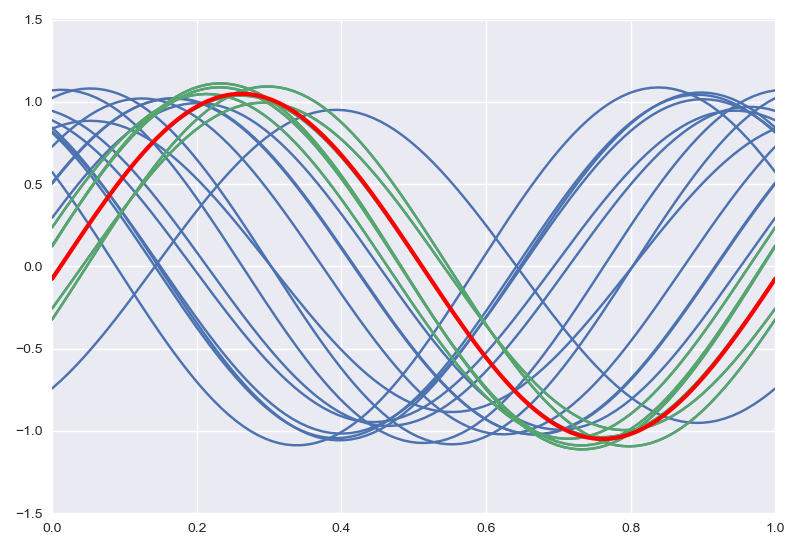
\includegraphics[width=7cm]{k-search}} \quad
	\subfigure[SBFIG:NNSEARCH2]{Radius-nearest neighbors}{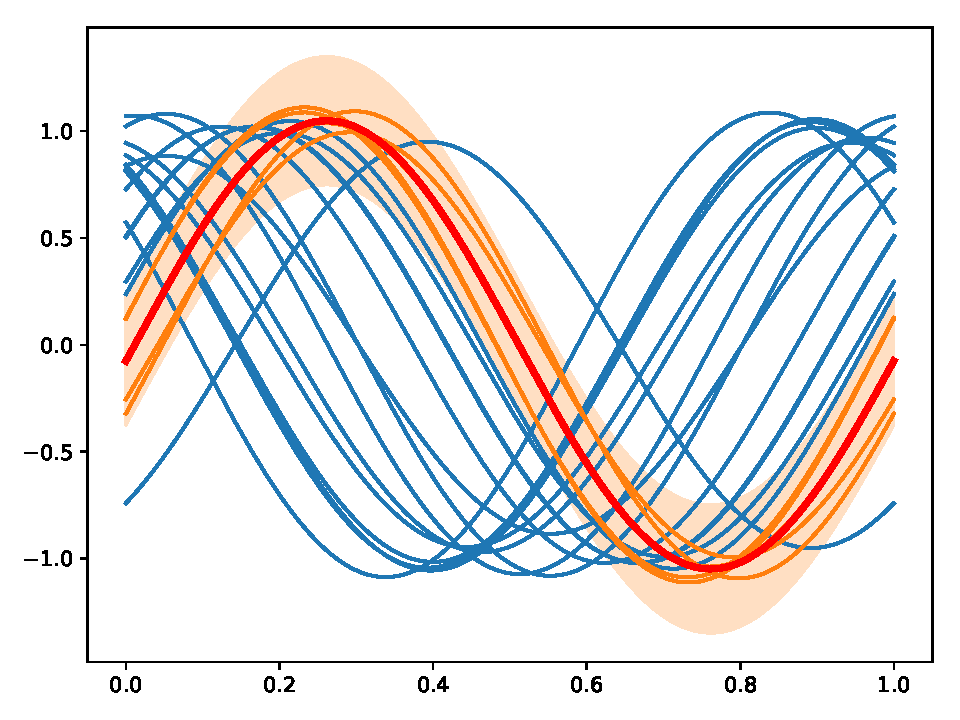
\includegraphics[width=7cm]{radius-search}}
\end{figure}

In the second variant, less used in practice, consisting of the radius neighbors
estimators, the neighborhood contains the samples $\mathcal{X}_i$ in the ball of
radius $r$ centered in $x$, i.e.
$k(x) = \{ \mathcal{X}_i : d(\mathcal{X}_i , x) \le r\}$. For instance, if we
use the distance $\mathbb{L}^\infty$, we may visualize $k(x)$ as the set of all
functions within a band  of radius $r$ around $x$.

In the figure \ref{FIG:NNSEARCH} there are shown the neighborhoods with these two different
approaches.

In practice, for the construction of the neighborhoods, the simplest solution is
 to perform a linear search, calculating the distances between $x$ and all the
 elements of the training set.

The naïve approach of the linear search may be improve using data structures
based on spatial indexes, such as ball trees \cite{Kumar2008}. However, the best
nearest-neighbor data structure for a given application will depend on the
dimensionality, size, and underlying structure of the data.
